% Options for packages loaded elsewhere
\PassOptionsToPackage{unicode}{hyperref}
\PassOptionsToPackage{hyphens}{url}
\documentclass[
  10pt,
  a4paper,
]{article}
\usepackage{xcolor}
\usepackage[margin=22mm]{geometry}
\usepackage{amsmath,amssymb}
\setcounter{secnumdepth}{-\maxdimen} % remove section numbering
\usepackage{iftex}
\ifPDFTeX
  \usepackage[T1]{fontenc}
  \usepackage[utf8]{inputenc}
  \usepackage{textcomp} % provide euro and other symbols
\else % if luatex or xetex
  \usepackage{unicode-math} % this also loads fontspec
  \defaultfontfeatures{Scale=MatchLowercase}
  \defaultfontfeatures[\rmfamily]{Ligatures=TeX,Scale=1}
\fi
\usepackage{lmodern}
\ifPDFTeX\else
  % xetex/luatex font selection
\fi
% Use upquote if available, for straight quotes in verbatim environments
\IfFileExists{upquote.sty}{\usepackage{upquote}}{}
\IfFileExists{microtype.sty}{% use microtype if available
  \usepackage[]{microtype}
  \UseMicrotypeSet[protrusion]{basicmath} % disable protrusion for tt fonts
}{}
\makeatletter
\@ifundefined{KOMAClassName}{% if non-KOMA class
  \IfFileExists{parskip.sty}{%
    \usepackage{parskip}
  }{% else
    \setlength{\parindent}{0pt}
    \setlength{\parskip}{6pt plus 2pt minus 1pt}}
}{% if KOMA class
  \KOMAoptions{parskip=half}}
\makeatother
\usepackage{graphicx}
\makeatletter
\newsavebox\pandoc@box
\newcommand*\pandocbounded[1]{% scales image to fit in text height/width
  \sbox\pandoc@box{#1}%
  \Gscale@div\@tempa{\textheight}{\dimexpr\ht\pandoc@box+\dp\pandoc@box\relax}%
  \Gscale@div\@tempb{\linewidth}{\wd\pandoc@box}%
  \ifdim\@tempb\p@<\@tempa\p@\let\@tempa\@tempb\fi% select the smaller of both
  \ifdim\@tempa\p@<\p@\scalebox{\@tempa}{\usebox\pandoc@box}%
  \else\usebox{\pandoc@box}%
  \fi%
}
% Set default figure placement to htbp
\def\fps@figure{htbp}
\makeatother
\setlength{\emergencystretch}{3em} % prevent overfull lines
\providecommand{\tightlist}{%
  \setlength{\itemsep}{0pt}\setlength{\parskip}{0pt}}
\usepackage{mathrsfs}
\newcommand{\Log}{\operatorname{Log}}
\usepackage{mathtools}
\usepackage{xurl}
\emergencystretch=3em
\setcounter{tocdepth}{1}
\newcommand{\Beta}{\mathrm{B}}
\DeclareUnicodeCharacter{00B2}{\ensuremath{^2}}
\DeclareUnicodeCharacter{00B1}{\ensuremath{\pm}}
\DeclareUnicodeCharacter{00D7}{\ensuremath{\times}}
\DeclareUnicodeCharacter{2192}{\ensuremath{\to}}
\DeclareUnicodeCharacter{21D2}{\ensuremath{\Rightarrow}}
\DeclareUnicodeCharacter{21A6}{\ensuremath{\mapsto}}
\DeclareUnicodeCharacter{2208}{\ensuremath{\in}}
\DeclareUnicodeCharacter{2209}{\ensuremath{\notin}}
\DeclareUnicodeCharacter{2212}{\ensuremath{-}}
\DeclareUnicodeCharacter{2227}{\ensuremath{\wedge}}
\DeclareUnicodeCharacter{2228}{\ensuremath{\vee}}
\DeclareUnicodeCharacter{2260}{\ensuremath{\ne}}
\DeclareUnicodeCharacter{2264}{\ensuremath{\le}}
\DeclareUnicodeCharacter{2265}{\ensuremath{\ge}}
\DeclareUnicodeCharacter{2297}{\ensuremath{\otimes}}
\DeclareUnicodeCharacter{00B3}{\ensuremath{^3}}
\DeclareUnicodeCharacter{2074}{\ensuremath{^4}}
\DeclareUnicodeCharacter{2076}{\ensuremath{^6}}
\DeclareUnicodeCharacter{03BB}{\ensuremath{\lambda}}
\DeclareUnicodeCharacter{03BC}{\ensuremath{\mu}}
\DeclareUnicodeCharacter{03B5}{\ensuremath{\epsilon}}
\DeclareUnicodeCharacter{03C4}{\ensuremath{\tau}}
\DeclareUnicodeCharacter{03A6}{\ensuremath{\Phi}}
\DeclareUnicodeCharacter{03B1}{\ensuremath{\alpha}}
\DeclareUnicodeCharacter{03C3}{\ensuremath{\sigma}}
\DeclareUnicodeCharacter{03B4}{\ensuremath{\delta}}
\DeclareUnicodeCharacter{03C0}{\ensuremath{\pi}}
\DeclareUnicodeCharacter{039B}{\ensuremath{\Lambda}}
\DeclareUnicodeCharacter{2202}{\ensuremath{\partial}}
\DeclareUnicodeCharacter{0393}{\ensuremath{\Gamma}}
\DeclareUnicodeCharacter{2205}{\ensuremath{\varnothing}}
\DeclareUnicodeCharacter{221E}{\ensuremath{\infty}}
\DeclareUnicodeCharacter{2200}{\ensuremath{\forall}}
\DeclareUnicodeCharacter{00B9}{\ensuremath{^1}}
\DeclareUnicodeCharacter{00B0}{\ensuremath{{}^\circ}}
\DeclareUnicodeCharacter{211D}{\ensuremath{\mathbb{R}}}
\usepackage{bookmark}
\IfFileExists{xurl.sty}{\usepackage{xurl}}{} % add URL line breaks if available
\urlstyle{same}
\hypersetup{
  hidelinks,
  pdfcreator={LaTeX via pandoc}}

\author{}
\date{}

\begin{document}

{
\setcounter{tocdepth}{3}
\tableofcontents
}
\section{Original-zeta endpoint sectors, zero motion and finite trace
return}\label{original-zeta-endpoint-sectors-zero-motion-and-finite-trace-return}

This proof retains the unfiltered theta density, both endpoint
exponentials, the complete Gamma multiplier, and the original zeta
function. It computes the difference between the sectorial continuation
of that density and the filtered arithmetic heat family. In particular,
finite dimension of the additive differential kernel does not identify
their zero divisors.

\subsection{1. Exact source and
coordinates}\label{exact-source-and-coordinates}

The complete programme source
\texttt{ENDPOINT\_\allowbreak{}SECTORIAL\_\allowbreak{}HEAT\_\allowbreak{}EXTENSION.\allowbreak{}tex}, ESH1--18, supplies
the two lateral continuations. Its full TeX is retained with this proof.
Its Gaussian and error-function integrations are reproduced below where
used. The original author heat kernel is Rodgers--Tao, \emph{The de
Bruijn--Newman constant is non-negative}, arXiv:1801.05914v5,
definitions \texttt{phidef} and \texttt{htdef},
\href{https://arxiv.org/src/1801.05914v5}{original author TeX}. UZ1--53
proves the complete multiplier and original-zeta return, including
exceptional germs;
\href{https://github.com/KokunoYumeto/zeta-function-research-reader/blob/a8e35be8f238913ae5bcbd8ad55a07d539b350f3/workbenches/splitzero-tandem/branches/tau-zero-prime-positivity/FAITHFUL_UNCOMPLETED_ZETA_HEAT.md}{public
proof}. The present calculations concern the additional endpoint
sectors, not a replacement of those definitions.

Throughout, (t\textgreater0) is the original real heat time and \[
\begin{aligned}
Z&=-2i(s-\tfrac12),& P(s)&=s(s-1),\\
A(s)&=\pi^{-s/2}\Gamma(s/2),& C(s)&=\tfrac12P(s)A(s),\\
\kappa(s)&=\frac{A'(s)}{A(s)}
=-\tfrac12\log\pi+\tfrac12\psi_\Gamma(s/2),&
\beta(s)&=\frac1s+\frac1{s-1}.
\end{aligned}\tag{SER1}
\] Here \(\psi_\Gamma=\Gamma'/\Gamma\). In particular
\(\kappa'=\psi_\Gamma'(s/2)/4\). All meromorphic equations below use
these full factors. Neither \(P\) nor \(A\) is suppressed.

Put \(\psi(x)=\sum_{n\ge1}e^{-\pi n^2x}\), and define \[
\begin{aligned}
\rho(u)&=8e^u\psi(e^{4u})-4e^{-u},\\
\mathcal L_t(s)&=8\int_0^\infty e^{tu^2+u}\psi(e^{4u})
                  \cosh((2s-1)u)\,du,\\
E_0(t,s)&=e^{-s^2/t},\qquad E_1(t,s)=e^{-(s-1)^2/t},
\qquad K_t=\sqrt{\pi/t}.
\end{aligned}\tag{SER2}
\] The term \(-4e^{-u}\) is the entire endpoint density on this
half-line. It is not erased from the following maps. The integral
defining \(\mathcal L\) is entire in \((t,s)\): on compact sets its
derivatives are bounded by powers of \(u\) times
\(M\exp(Tu^2+(2R+2)u-ce^{4u})\). This integrable majorant follows by
splitting the Gaussian exponent in the sum over \(n\).

For any complex \(a\), define \[
F_+(t,a)=-i\int_0^\infty e^{-tv^2+iav}\,dv,
\qquad
F_-(t,a)=i\int_0^\infty e^{-tv^2-iav}\,dv.
\tag{SER3}
\] These are entire in \(a\). They are precisely the upper and lower
\(q=-t\) boundary values of
\(\sqrt\pi\,e^{a^2/(4q)}\operatorname{erfc}(a/(2\sqrt q))/(2\sqrt q)\):
this follows by completing the square, first for real positive \(q\),
and continuing its entire error-function expression to
\(\sqrt q=\pm i\sqrt t\). The full Gaussian Fourier integral gives \[
F_+(t,a)+F_+(t,-a)=-iK_t e^{-a^2/(4t)},
\qquad F_+-F_-=-iK_t e^{-a^2/(4t)}.
\tag{SER4}
\] The Gaussian Fourier identity follows, for real \(a\), by
differentiating its integral in \(a\) and integrating by parts,
obtaining derivative \(-a/(2t)\) times the integral, and evaluating at
zero. Both sides are entire in \(a\), which proves the stated complex
identity.

The two retained raw integrals and their original-zeta coordinates are
\[
\begin{aligned}
\mathcal I_\pm(t,s)
 &=\mathcal L_t(s)-2F_\pm(t,2s)-2F_\pm(t,2-2s),\\
f_\pm(t,s)&=A(s)^{-1}\mathcal I_\pm(t,s).
\end{aligned}\tag{SER5}
\] For each positive \(t\), \(\mathcal I_\pm\) and \(f_\pm\) are entire
in \(s\). The reciprocal Gamma function is entire. By contrast, the
original-zeta filtered family is the meromorphic function \[
\begin{aligned}
\Phi(u)&=\sum_{n\ge1}
 (2\pi^2n^4e^{9u}-3\pi n^2e^{5u})e^{-\pi n^2e^{4u}},\\
H_t(Z)&=\int_0^\infty e^{tu^2}\Phi(u)\cos(Zu)\,du,\\
\zeta_t(s)&=\frac{16H_t(-2i(s-\tfrac12))}{P(s)A(s)},
\qquad \zeta_0=\zeta.
\end{aligned}\tag{SER6}
\] The full local comparison of (SER5) and (SER6) is therefore necessary
even before comparing zeros.

\subsection{2. A common part and both retained endpoint
sectors}\label{a-common-part-and-both-retained-endpoint-sectors}

Define the following actual entire function for \(t>0\): \[
\begin{aligned}
J_t(s)
 &=\mathcal L_t(s)-2F_+(t,2s)+2F_+(t,2(s-1))\\
 &=\mathcal L_t(s)+2i\int_0^\infty e^{-tv^2}
       \big(e^{2isv}-e^{2i(s-1)v}\big)\,dv.
\end{aligned}\tag{SER7}
\] Substitution of (SER4), with no limiting argument, proves \[
\begin{aligned}
\mathcal I_+&=J_t+2iK_t E_1,\\
\mathcal I_-&=J_t-2iK_t E_0,\\
f_+-f_-&=2iK_t A^{-1}(E_0+E_1).
\end{aligned}\tag{SER8}
\] These equations retain both endpoint terms, including their signs and
the factor \(A^{-1}\). The triangular map on triples \[
(J,E_0,E_1)\longmapsto(J+2iK_t E_1,E_0,E_1)
\tag{SER9}
\] has inverse \((I,E_0,E_1)\mapsto(I-2iK_t E_1,E_0,E_1)\); the lower
branch has the corresponding inverse with \(-2iK_t E_0\). Thus the
augmented data are exactly recoverable. Forgetting the last two
coordinates is a different map.

On every compact set \(K\subset\{\Im s>0\}\), the integrand in (SER7),
after any finite number of \(s\)- or right \(t\)-derivatives at \(t=0\),
is bounded by a polynomial in \(v\) times \(e^{-2\delta v}\), where
\(\delta=\min_K\Im s>0\). Dominated convergence proves a locally uniform
\(C^\infty\) extension to \(t=0+\). Since
\(\int_0^\infty e^{2isv}\,dv=-1/(2is)\), its value is \[
J_0(s)=\mathcal L_0(s)-\frac1s+\frac1{s-1}=A(s)\zeta(s),
\quad \Im s>0.
\tag{SER10}
\] For \(0<\Re s<1\) this is the original theta Mellin identity. The two
sides are holomorphic on the connected upper half-plane, so their
equality extends there by the identity theorem. Define \(u_t=A^{-1}J_t\)
on this domain, including \(u_0=\zeta\). This is an explicitly augmented
common-part coordinate from (SER9); it is not a declaration that the
endpoint terms vanished.

Differentiating the integrals gives the three exact equations \[
\partial_t J_t=\tfrac14\partial_s^2J_t,
\quad
\partial_t u_t=\tfrac14(\partial_s+\kappa)^2u_t,
\quad
\partial_t\zeta_t=\tfrac14(\partial_s+\kappa+\beta)^2\zeta_t.
\tag{SER11}
\] They hold for \(t>0\); the first two hold in right derivatives at
zero on the upper half-plane. The last follows by differentiating
(SER6). For example \(\partial_s^2 e^{2isv}/4=-v^2e^{2isv}\), which
checks the original heat-time sign in (SER11).

\subsection{3. Smooth return with a divergent time
series}\label{smooth-return-with-a-divergent-time-series}

For every integer \(k\ge0\), evaluating the exponential moments gives \[
\left.\partial_t^k J_t(s)\right|_{0+}
=\left.\partial_t^k\mathcal L_t(s)\right|_0
+\frac{(2k)!}{4^k}
 \left(\frac1{(s-1)^{2k+1}}-\frac1{s^{2k+1}}\right).
\tag{SER12}
\] Indeed \(\int_0^\infty v^{2k}e^{2isv}dv=(2k)!/(-2is)^{2k+1}\), by
repeated integration by parts; multiplying by \(2i(-1)^k\) produces
exactly the two signs in (SER12).

For fixed \(s\) with \(\Im s>0\), the Taylor series of \(J_t(s)\) at
\(0+\) has radius of convergence zero. Here is a proof including
possible equal endpoint distances. If \(|s|\ne|s-1|\), the nearer
endpoint term in (SER12) dominates the other geometrically. The \(k\)-th
root of \((2k)!/(4^k k!)\) tends to infinity: it is at least
\((k!)^{1/k}/4\), and the last \(\lfloor k/2\rfloor\) factors of \(k!\)
already prove divergence of this lower bound. If \(|s|=|s-1|\), write
\(s=R e^{i\theta}\), \(0<\theta<\pi/2\); then
\(s-1=R e^{i(\pi-\theta)}\) and the difference in (SER12) is \[
-2R^{-2k-1}\cos((2k+1)\theta).
\tag{SER13}
\] For every real \(x\),
\(|\sin(2\theta)|\le|\cos x|+|\cos(x+2\theta)|\), by the sine
subtraction identity. At least one of each consecutive pair of cosine
factors in (SER13) is therefore at least \(\sin(2\theta)/2>0\) in
absolute value. The same infinite limsup of coefficient roots follows.
Finally the \(k\)-th roots of the Taylor coefficients of
\(\mathcal L_t(s)\) tend to zero because it is entire in \(t\). They
cannot cancel that subsequence. The reciprocal \(A(s)\) is a nonzero
constant at this fixed upper-half-plane point, so the time Taylor series
of \(u_t(s)\) also has radius zero.

This divergence has an explicit remainder object. For \(t\ge0\), the
remainder of the exponential after its first \(N\) terms satisfies
\(|e^{-tv^2}-\sum_{k=0}^{N-1}(-tv^2)^k/k!|\le t^Nv^{2N}/N!\), by the
integral Taylor remainder. Thus, on \(\Im s\ge\delta>0\), the
endpoint-integral remainder in (SER7) is bounded by \[
\frac{4t^N(2N)!}{N!(2\delta)^{2N+1}}.
\tag{SER14}
\] The entire \(\mathcal L\) remainder is retained separately. Equations
(SER12)--(SER14) define and bound the actual asymptotic jet. They do not
turn it into a convergent heat-time expansion.

\subsection{4. Reflection and the full differential
return}\label{reflection-and-the-full-differential-return}

Define \(g^\#(s)=\overline{g(1-\bar s)}\) at real \(t\). Conjugating the
two legs of (SER7) and using the even, real kernel in \(\mathcal L\)
gives \[
\begin{aligned}
J_t^\#&=J_t,&
J_t(1-s)-J_t(s)&=2iK_t(E_1-E_0),\\
\mathcal I_\pm(1-s)&=\mathcal I_\pm(s),&
\mathcal I_+^\#&=\mathcal I_-.
\end{aligned}\tag{SER15}
\] The second equation also follows directly by subtracting the two
versions of (SER8). For the original-zeta coordinates one must retain,
for example, \(A^\#u_t^\#=Au_t\) and \(A^\# f_+^\#=Af_-\). These are the
exact Gamma-twisted reflections; no factor-free reflection of \(f_+\) is
asserted.

The complete source filter, in the original \(Z\) coordinate, is \[
N_t=-\frac{1+Z^2-2t-4tZ\partial_Z+4t^2\partial_Z^2}{64}.
\tag{SER16}
\] To check its boundary terms, integrate \(\rho''\) twice against
\(e^{tu^2}\cos Zu\). The result is \(-\rho'(0)-(Z-2t\partial_Z)^2I\).
Poisson differentiation of the original Gaussian theta identity at one
gives \(\psi'(1)=-\psi(1)/4-1/8\), hence
\(\rho'(0)=8\psi(1)+32\psi'(1)+4=0\). Direct differentiation of the sum
defining \(\rho\) gives \((\rho''-\rho)/64=\Phi\). These computations
first prove \(N_tI=H_t\) on the convergent negative-time domain, and
then on each sector by continuation of the same error-function formulas.
For the separate endpoint and summable terms, with
\(B=(F(2s)+F(2-2s))/2\), the boundary evaluation is \[
N_tB=-\frac1{64},\qquad
N_t\mathcal L_t=H_t-\frac1{16},\qquad
N_t(\mathcal L_t-4B)=H_t.
\tag{SER17}
\] Thus neither of the separate boundary constants is silently set to
zero.

In original \(s\) coordinates, (SER16)--(SER17) become \[
\begin{aligned}
\mathcal P_t f
 &=f+\frac{t}{2P}f
 +\frac{t(2s-1)}{2P}(\partial_s+\kappa)f
 +\frac{t^2}{4P}(\partial_s+\kappa)^2f,\\
\zeta_t&=\mathcal P_t f_+=\mathcal P_t f_-=\mathcal P_t u_t.
\end{aligned}\tag{SER18}
\] For the last equality, substitution of \(E_0,E_1\) into
\([P+t/2]+t(2s-1)\partial_s/2+t^2\partial_s^2/4\) gives zero exactly. In
particular the factors \(K_t\) do not change this spatial annihilation.
The equation is an identity of meromorphic functions, including the full
\(P A\) denominator. At exceptional points it is interpreted by the full
Laurent germs, not by dividing their values.

\subsection{5. A domain where the endpoint sectors remove nearby
zeros}\label{a-domain-where-the-endpoint-sectors-remove-nearby-zeros}

Consider the explicit open domain \[
\mathcal W=\{s=\sigma+i\gamma:
\gamma>\max(|\sigma|,|\sigma-1|)\}.
\tag{SER19}
\] For a compact \(K\subset\mathcal W\), define
\(\eta=\min_K\{\gamma^2-\sigma^2,\gamma^2-(\sigma-1)^2\}>0\). The
locally uniform convergence in (SER10) bounds \(|J_t|\le M_K\) for
\(0\le t\le t_K\). Equation (SER8) now gives, on all of \(K\), \[
|\mathcal I_\pm(t,s)|\ge
2\sqrt{\pi/t}\,e^{\eta/t}-M_K>0
\quad\hbox{for sufficiently small positive }t.
\tag{SER20}
\] The multiplier \(A^{-1}\) is a unit on \(K\), so neither raw \(f_+\)
nor raw \(f_-\) has a zero there at such times.

At every zero \(\rho\in\mathcal W\) of the original \(\zeta\), choose a
closed disc \(D\subset\mathcal W\) containing no other zero and with no
boundary zero. The two families \(u_t\) and \(\zeta_t\) converge
uniformly to \(\zeta\) on \(D\), by (SER10) and the entire-time integral
(SER6). On \(\partial D\) their differences from \(\zeta\) are therefore
smaller than \(|\zeta|\) for sufficiently small \(t>0\). Rouché's
theorem proves that each has exactly \(\operatorname{ord}_\rho\zeta\)
zeros in \(D\), counted with multiplicity. Equation (SER20) proves that
each lateral raw family has none there. This is an evaluated difference
of zero divisors on the stated domain. No claim about all zeros follows
from a finite-dimensional additive kernel alone.

\subsection{6. Exact first variation and every finite
contour}\label{exact-first-variation-and-every-finite-contour}

Set \(D_A=\partial_s+\kappa\). Since \(\beta'+\beta^2=2/P\), direct
expansion of (SER11) proves \[
\frac14(D_A+\beta)^2-\frac14D_A^2
=\frac\beta2D_A+\frac1{2P}.
\tag{SER21}
\] The \(1/(2P)\) term is retained even though it vanishes after
evaluation on a zero of \(\zeta\).

For a simple original zero \(\rho\) in the upper half-plane, its local
zero in \(u_t\) has a right derivative by the real implicit-function
theorem applied to the locally holomorphic family and (SER10). Its
counterpart in \(\zeta_t\) is analytic in time. The derivatives are \[
\begin{aligned}
v_A&=-\frac14\left(\frac{\zeta''(\rho)}{\zeta'(\rho)}+2\kappa(\rho)\right),\\
v_C&=-\frac14\left(\frac{\zeta''(\rho)}{\zeta'(\rho)}+2\kappa(\rho)+2\beta(\rho)\right),\\
v_C-v_A&=-\frac12\left(\frac1\rho+\frac1{\rho-1}\right).
\end{aligned}\tag{SER22}
\] These are not velocities of \(f_\pm\), whose local zero absence was
computed in (SER20). For \(\rho=1/2+x+iy\), multiplication by the
conjugate denominator yields the exact real part \[
\Re(v_C-v_A)=
-\frac{x(x^2+y^2-1/4)}{|\rho(\rho-1)|^2}.
\tag{SER23}
\] Both possible signs and the zero cases remain. In particular the
difference is purely imaginary at \(x=0\). Equation (SER15), together
with uniqueness of a simple zero near its starting point, shows that a
simple critical-line zero of \(u_t\) stays on that line for sufficiently
small real \(t\). The same local conclusion holds for \(\zeta_t\). This
is a local statement until a collision or loss of the chosen
neighbourhood; no global positivity is inferred.

For arbitrary multiplicity, use the logarithmic derivatives away from
zeros, rather than choosing individual differentiable roots. Equations
(SER11) and (SER21) give \[
\left.\partial_t\left(
\frac{\partial_s\zeta_t}{\zeta_t}
-\frac{\partial_su_t}{u_t}\right)\right|_{0+}
=\partial_s\left[
\frac\beta2\left(\frac{\zeta'}\zeta+\kappa\right)+\frac1{2P}\right].
\tag{SER24}
\] At an original zero \(\rho\) of multiplicity \(m_\rho\), its
principal part is exactly \(-m_\rho\beta(\rho)/(2(s-\rho)^2)\); there is
no simple pole. This follows by expanding the bracket as
\(m_\rho\beta(\rho)/(2(s-\rho))+\text{holomorphic}\) before
differentiating.

Let \(D\) be any bounded domain with piecewise smooth positively
oriented boundary, with closure in the upper half-plane and no zero of
\(\zeta\) on its boundary. Let \(a(s)\) be holomorphic on a
neighbourhood of \(\overline D\). All sufficiently small \(t\ge0\)
retain a zero-free boundary. The argument principle and its locally
uniform right derivative prove \[
\begin{aligned}
\left.\frac d{dt}\right|_{0+}
\bigg[
 \sum_{\rho_t\in D}m_{\rho_t}a(\rho_t)
 -\sum_{\eta_t\in D}m_{\eta_t}a(\eta_t)
\bigg]
 =-\frac12\sum_{\rho\in D}m_\rho\beta(\rho)a'(\rho),
\end{aligned}\tag{SER25}
\] where the first sum uses \(\zeta_t\) and the second uses \(u_t\). To
verify it directly, integrate (SER24) against \(a(s)/(2\pi i)\); the
residue of its double pole is \(-m_\rho\beta(\rho)a'(\rho)/2\). This
proof includes all multiple zeros. It neither differentiates them
separately nor exchanges a derivative with an infinite zero sum.

\subsection{7. Growth, retained support and the receiving
calculations}\label{growth-retained-support-and-the-receiving-calculations}

For each fixed positive \(t\), the functions
\(J_t,\mathcal I_\pm,f_\pm\) are of order at most two. A sufficient
direct bound on the integral in (SER7) is \[
\int_0^\infty e^{-tv^2+2|\Im s|v}dv
\le\sqrt{\pi/t}\,e^{|\Im s|^2/t}.
\tag{SER26}
\] For \(\mathcal L_t\), its defining double-exponential majorant gives
\(\log^+|\mathcal L_t(s)|=O_t((1+|s|)\log(2+|s|))\). For completeness,
absorb \(tu^2+u\) into one quarter of the Gaussian exponent plus a
constant. The supremum of \(2Ru-(\pi/2)e^{4u}\) on \(u\ge0\) is bounded
by \(O(R\log(2+R))\); leave another quarter of the exponential to
integrate in \(u\). This proves the asserted bound. The elementary
reciprocal Gamma product UZ6 gives
\(\log^+|A^{-1}(s)|=O((1+|s|)\log(2+|s|))\), so it does not increase the
order upper bound. These are upper bounds; they do not assert a
quadratic lower bound for zero counts, or divergence of a particular
quadratic-decay trace. In particular, a genus-one trace domain from the
filtered family cannot be transferred solely by invoking finite
dimension of (SER18)'s kernel.

All source comparisons are made over the actual fixed coefficient base.
For a support semilattice \(L\) with least support \(\bot\) and greatest
support \(\top\), its carrier here is \[
G_L(V)=\{(0,\lambda):\lambda\in L\}
\ \cup\ \{(v,\top):v\in V\setminus\{0\}\}.
\tag{SER27}
\] In particular \(\tau=(0,\bot)\) and \(e=(0,\top)\) stay distinct.
Every linear function-space map in this proof has the explicit labelled
extension \((v,\top)\mapsto(Tv,\top)\), while each lower-support point
\((0,\lambda)\) stays that very point. A vanishing top amplitude
therefore lands at \(e\), not at \(\tau\). The scalar coefficient-base
morphism is the identity, with the identity pullback on its prime
spectrum. No semiring homomorphism, or new spectral pullback, is
inferred merely from linearity of the differential filter. Endpoint
coordinates in (SER9) and lower-support points in (SER27) are both
retained and are not identified with one another.

The exact effects on the earlier calculations are now specified. UZ's
actual filtered original-zeta equation is the third equation of (SER11),
with the full \(\beta\) contribution. Replacing it by the unfiltered
return would remove the evaluated operator (SER21) and change the finite
trace by (SER25). Its positive-time lateral branches require (SER8);
their zeros cannot be identified with the filtered zeros in the domain
(SER19). Any use of the unfiltered time jets must use the remainder
(SER14), because their Taylor radius is zero. The finite-contour trace
formula is proved at the domain stated in (SER25); no unproved global
contour limit or positivity conclusion is included.

\begin{figure}
\centering
\pandocbounded{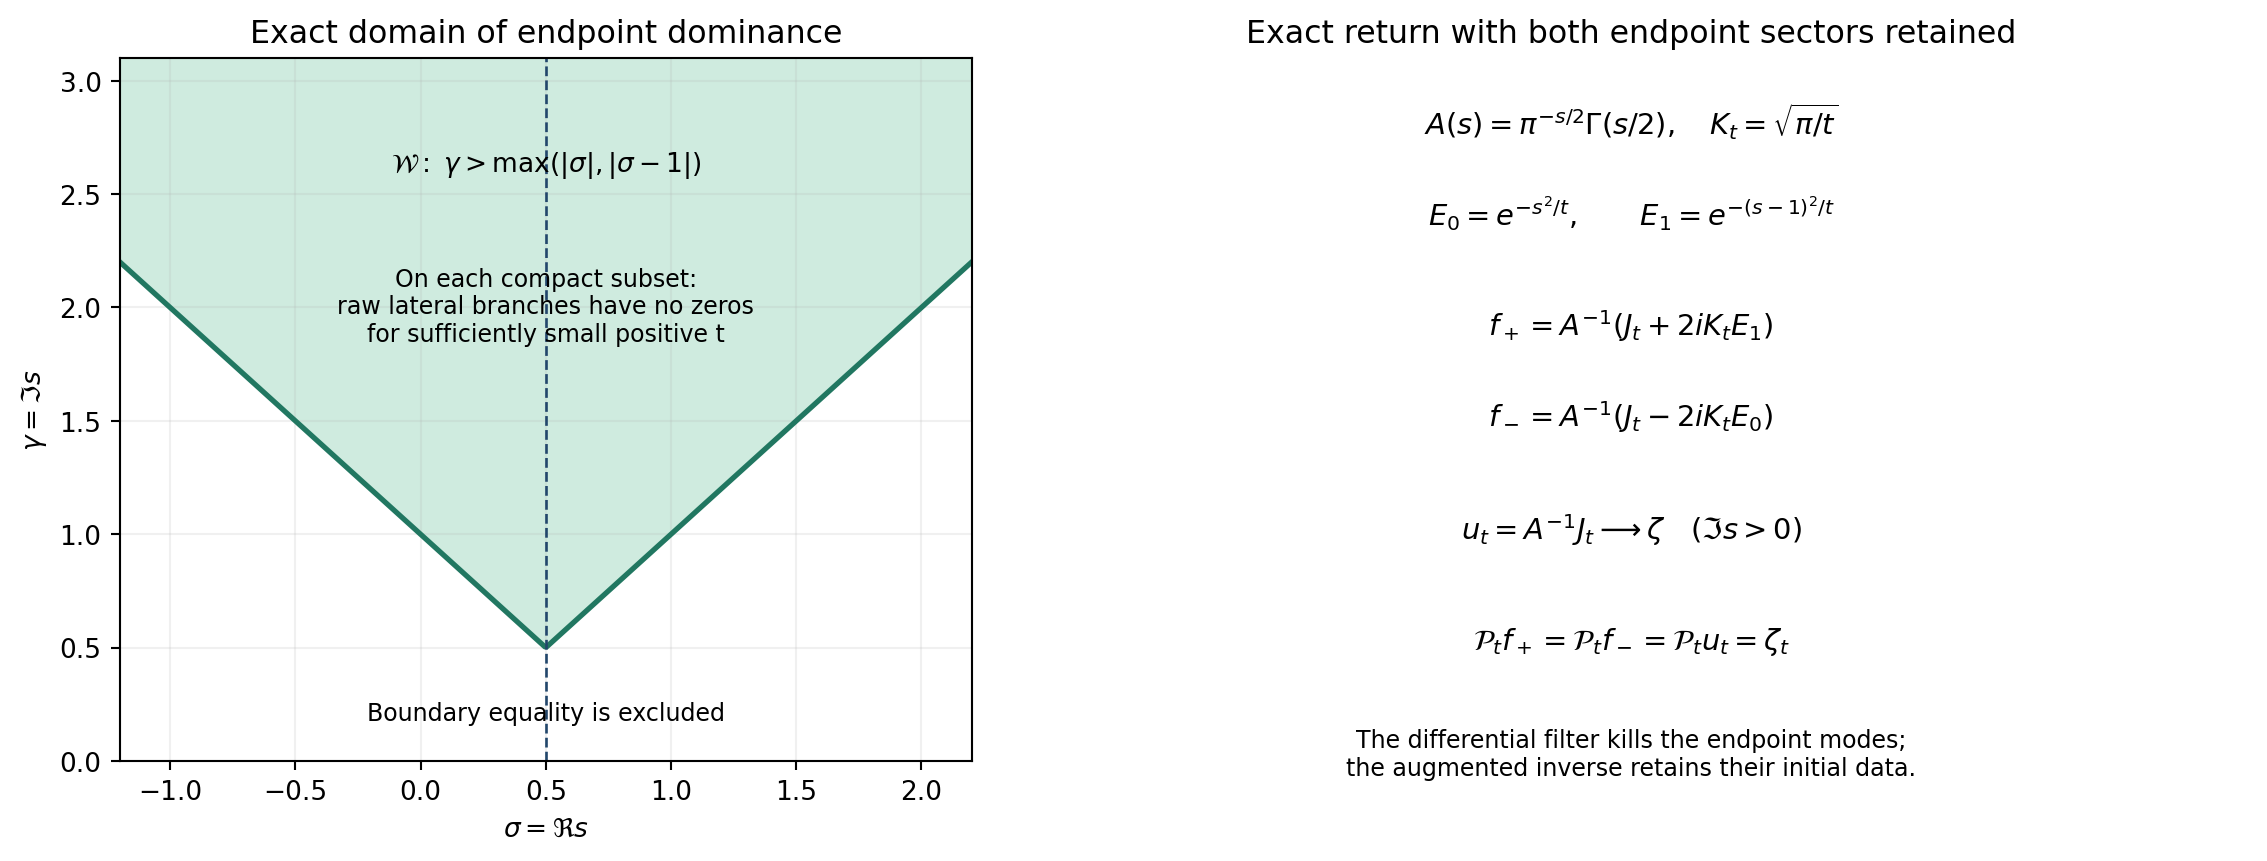
\includegraphics[keepaspectratio,alt={Exact endpoint dominance domain and retained maps. SER8--10 and SER18--20 prove every displayed factor and the compact-set zero exclusion. This diagram does not plot zeta zeros or assert one uniform time bound for the unbounded domain. SFT12--22 gives the complete inverse with its original initial data. The source is the full ESH1--18 comparison and the original Rodgers--Tao kernel cited in SER1.}]{sectorial_endpoint_return.png}}
\caption{Exact endpoint dominance domain and retained maps. SER8--10 and
SER18--20 prove every displayed factor and the compact-set zero
exclusion. This diagram does not plot zeta zeros or assert one uniform
time bound for the unbounded domain. SFT12--22 gives the complete
inverse with its original initial data. The source is the full ESH1--18
comparison and the original Rodgers--Tao kernel cited in SER1.}
\end{figure}

\subsection{Endpoint-resonant detector and its original-time
boundary}\label{endpoint-resonant-detector-and-its-original-time-boundary}

The complete \href{ENDPOINT_RESONANT_ZERO_DETECTION.md}{ERD1--50 proof}
proves that the actual endpoint-resonant cosine transform at t=1/32 is
nonzero throughout the closed critical strip, uniformly in height. It
retains the full original zeta product at both shifted arguments, every
exceptional germ and an explicit phase bound. The same source has a zero
complete right-time Taylor jet at time zero: ERD40--50 retains the exact
exponential factor, constructs its nonzero nonnilpotent flat germ,
evaluates the dual-number jet map, and supplies the positive-time
inverse with its analytic coordinate. Vanishing of these time jets does
not discard the positive-time detector.

The full \href{ENDPOINT_PAIR_TRANSPORT_AND_WEIL_MATRIX.md}{EPM1--47
proof} calculates the cosine/sine pair's coupled original-time
transport, its inverse, both endpoint argument maps and their
common-zero set. The sine source is odd; EPM19--21 constructs a split
extension of the even prime quotient rather than inserting that source
into the old domain. EPM28--31 retains every finite original
trivial-zero entry and the Gamma boundary. EPM43--47 puts the
companion's certified50\textless K(0)\textless64 for the actual cosine
test into the exact global translated criterion RH iff
\textbar K(a)\textbar\textless=K(0) for every a\textgreater=0. Its
positive diagonal does not prove the global inequality. The complete
arithmetic certificate source, executable and independent tail proof are
included unchanged.

\end{document}
